% Capítulo 2 - vFinal 1.0 - 05/07/2018
\chapter{Conceitos Relacionados}
\label{cap:cap2}

Este capítulo aborda os conceitos e técnicas que proporcionam a compreensão dos capítulos a seguir. A Seção \ref{cap2:energyDriven} introduz o conceito da computação dirigida aos fatores energéticos, tema originador do trabalho. Na Seção \ref{cap2:iot}, apresento a visão geral sobre Redes IoT e dispositivos que compõe o alvo das iniciativas propostas. Por sua vez, na Seção \ref{cap2:throttling} encontram-se os conceitos ligados ao padrão throttling, seu conceito e sua aplicação. A intenção de uso de um modelo taxonômico esta fundamentada na Seção \ref{cap2:taxonomia}.

\section{Energy-Driven Computing}
\label{cap2:energyDriven}

Um sistema dirigido à energia (\textit{Energy-Driven}), é todo aquele que os fatores energéticos intrínsecos a ele são tratados como primários, desde concepção, gerenciamento e sua operação \cite{merrett_energy-driven_2017}. Computação dirigida a estes fatores, ditos energéticos, deve considerar fundamentalmente a disponibilidade energética pois primariamente precisam carregar a capacidade de adaptação as dinâmicas de captação de energia. Este paradigma tem como objetivo evidenciar as características energéticas, em potencial a respeito de dispositivos que por quaisquer motivos, não podem estar conectados diretamente em uma infraestrutura capaz de fornecer energia regularmente. 

Para tal, caso necessário, dispositivos podem operar coletando recursos disponíveis no ambiente. Coleta de energia refere-se a capacidade de um dispositivo em capturar e converter recursos energéticos do meio e converte-los de modo a prolongar sua vida útil mitigando um cenário de escassez energética \cite{sudevalayam_energy_2011}. 

Ainda, no trabalho de \cite{sliper_energy-driven_2020} é importante destacar como os mecanismos de coleta energética e sua dinâmica são dispostos. É proposto uma organização em três categorias distintas: Neutra-Energética \ac{EN}, Neutra-Força ou Neutra em Consumo \ac{PNO} e por fim, Operações Intermitentes.

\subsection{Operação Energy-Neutral}
Uma operação neutra-energética \cite{kansal_power_2007}, cobre as dinâmicas dos sistemas com coleta de energia do ambiente por meio de um \textit{buffer}, uma bateria recarregável ou super capacitor capaz de armazenar parte da energia coletada. Este recurso, se encontra disposto entre a entrada energética e sua demanda, atuando secundariamente quando a energia disponibilizada não seria suficiente para manter seus critérios de qualidade de serviço \textit{QoS}.

Apesar de inicialmente ser previsto um cenário de uso onde apenas a fonte energética e o dispositivo estivessem presentes, é comum o fato dos mecanismos que buscam esse tipo de operação recorrer a presença deste componente intermediário capaz de armazenar energia e disponibiliza-la para uso. Sendo assim, na Figura \ref{fig:cap2harveststoreuse} temos a visão geral em blocos de um subsistema responsável pelos recursos energéticos.

\begin{figure}[H]
	\centering
	\caption{Diagrama de blocos subsistema energético para operação neutro-energética.}
	\label{fig:cap2harveststoreuse}
	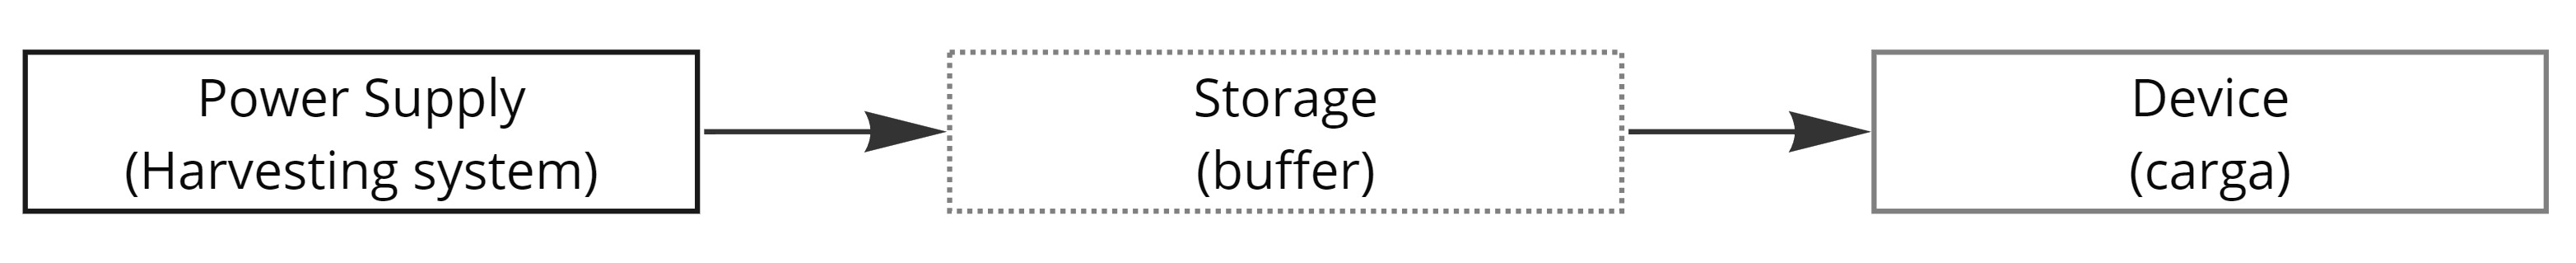
\includegraphics[width=0.7\linewidth]{Imagens/cap2/cap2harvest_store_use}	
	
	Fonte: adaptado de \cite{sudevalayam_energy_2011} 
\end{figure}



As operações dessa natureza carregam dois princípios que são apresentados no trabalho seminal de \cite{kansal_power_2007}: Manter-se operacional mesmo em cenários onde a quantidade de energia coletada fosse durante muito tempo, inferior ao necessário e como garantir que, dado um ambiente de coleta é possível obter máxima de performance ignorando variações da energia coletada. 

É importante destacar ainda que este modelo de operação serve como base para os diversos avanços em computação dirigida a energia. Ao apresentar os conceitos de operação-neutra, a teoria de coleta energética e seus questionamentos, carrega intrinsecamente as bases do que posteriormente foi detalhado como \acf{PNO} sendo utilizado inclusive como referencia no seminal \cite{merrett_energy-driven_2017} introdutório do tema.



\subsection{Operação Power-Neutral}
\subsection{Operação Intermitente}



\begin{itemize}
	% Definição, o que é? 
	
	% Relevancia dos conceitos
	\item Discussão sobre a relevância desses conceitos em ambientes tecnológicos, especialmente em sistemas IoT.
\end{itemize}

\section{Redes IoT}
\label{cap2:iot}
\begin{itemize}
	\item Revisão da literatura sobre os diferentes componentes de consumo de energia em dispositivos IoT, incluindo processadores, transmissores de rádio, sensores e circuitos de controle de energia.
	\item Abordagens e modelos para estimar e prever o consumo de energia em dispositivos IoT.
	\item Leitura Pertinente: referencia de estudos sobre técnicas e estratégias para otimizar o consumo de energia em dispositivos IoT, assim como esquemas de gerenciamento de energia em redes IoT.
\end{itemize}

\section{Throttling: Padrão de Controle de Comportamento em Ambientes Distribuídos}
\label{cap2:throttling}
\begin{itemize}
	\item Conceituação de throttling e sua aplicação em sistemas computacionais distribuídos.
	\item Exploração de diferentes técnicas de throttling e seus efeitos sobre o consumo de energia e desempenho do sistema em cenários como redes IoT.
	\item Leitura Pertinente: referencias de estudos que aborda o uso de throttling em ambientes distribuídos e sua influência na eficiência energética.
\end{itemize}

\section{Taxonomia}
\label{cap2:taxonomia}
\begin{itemize}
	\item Introdução à Taxonomia:
	 \begin{comment}
		 A taxonomia refere-se à classificação e organização sistemática de elementos 	dentro de um campo específico de estudo. No contexto das redes IoT, a taxonomia pode ser aplicada para classificar dispositivos, protocolos de comunicação, aplicações e outros elementos relacionados às redes IoT com base em suas características, funcionalidades e requisitos específicos.
	\end{comment}
	\item Benefícios da Taxonomia: 
	\begin{comment}
		A utilização de uma taxonomia clara e abrangente em redes IoT pode trazer uma série de benefícios, incluindo a padronização de terminologias, a simplificação da análise e comparação de sistemas, a identificação de lacunas de pesquisa e a facilitação da comunicação entre os profissionais do campo.
	\end{comment}
	
	\item Desafios e Considerações:
	\begin{comment}
		Embora a taxonomia ofereça muitos benefícios, sua criação e manutenção podem ser desafiadoras devido à natureza dinâmica e em constante evolução das redes IoT. Além disso, é importante considerar as diferentes perspectivas e abordagens para desenvolver uma taxonomia que seja abrangente, relevante e flexível o suficiente para atender às diversas necessidades e contextos das redes IoT.
	\end{comment}
	
	\item Aplicações Práticas: 
	\begin{comment}			
		A taxonomia pode ser aplicada em uma variedade de contextos em redes IoT, 	incluindo a classificação de dispositivos e sensores, a categorização de protocolos de comunicação, a organização de aplicações e serviços, e a definição de métricas de desempenho e segurança.
	\end{comment}
\end{itemize}

\section{Considerações Finais}
 \label{cap2:consideracoesFinais}
\begin{itemize}
	\item Síntese dos principais pontos discutidos no referencial teórico.
	\item Apontamento para a relevância desses conceitos na elaboração e implementação do projeto proposto.
\end{itemize}
	

\blindtext[2]
